\documentclass[12pt]{article}
\usepackage[T1]{fontenc}
\usepackage[utf8]{inputenc}
\usepackage[fleqn]{amsmath}
\usepackage{tikz}
\usetikzlibrary{arrows.meta}
\usetikzlibrary{calc}
\usetikzlibrary{ decorations.markings}
\usetikzlibrary{positioning}

\begin{document}

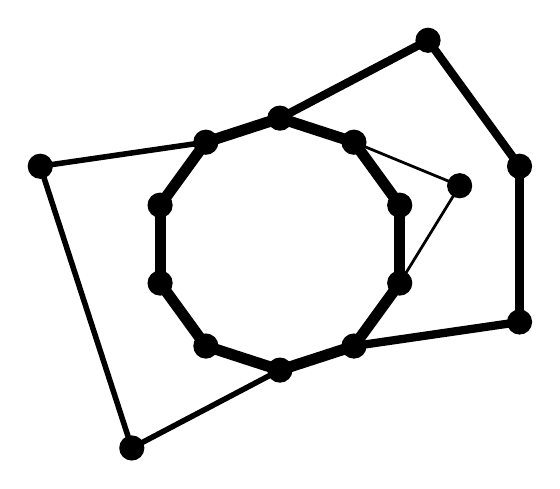
\begin{tikzpicture}[scale=2]
				\foreach \i in {1, 2, 3, 4, 5, 6, 7, 8, 9, 10}
				{
					\coordinate (V1\i) at (90 - \i * 360/10 + 360/10:0.8);
					\path[fill=black] (V1\i) circle (0.08);
				}
				
				\foreach \i/\j in {1/2, 2/3, 3/4, 4/5, 5/6, 6/7, 7/8, 8/9, 9/10, 10/1}
				{
					\path[draw][line width=4pt](V1\i) -- (V1\j);
				}
				
				% ucho 4 krawedzie
				\foreach \i in {1, 2, 3}
				{
					\coordinate (V2\i) at (90 - \i * 360/10 :1.6);
					\path[fill=black] (V2\i) circle (0.08);
				}
				\foreach \i/\j in {1/2, 2/3}
				{
					\path[draw][line width=3pt](V2\i) -- (V2\j);
				}
				\path[draw][line width=3pt](V11) -- (V21);
				\path[draw][line width=3pt](V15) -- (V23);
				
				% ucho 3 krawedzie
				\foreach \i in {1, 2}
				{
					\coordinate (V3\i) at (90 + \i * 360/5 :1.6);
					\path[fill=black] (V3\i) circle (0.08);
				}
				\path[draw][line width=2pt](V31) -- (V32);
				\path[draw][line width=2pt](V110) -- (V31);
				\path[draw][line width=2pt](V16) -- (V32);
				
				% ucho 2 krawedzie
				\coordinate (V41) at (90 - 2 * 360/10 :1.2);
				\path[fill=black] (V41) circle (0.08);
				\path[draw][line width=1pt](V12) -- (V41);
				\path[draw][line width=1pt](V14) -- (V41);
				
			\end{tikzpicture}

\end{document}